\chapter{More Hausdorff type axioms}

There are other $(T_2)$-type axioms for frames.
The aim of this chapter is to give a confrontation of the Dowker-Strauss
definition with axioms proposed by other pointless topologists.

\section{Variants of (DS-Haus)}

\subsection{The axiom of Johnstone and Sun Shu-Hao}

Johnstone and Sun Shu-Hao \cite{johnstone-shu-hao} suggest the axiom
\[
  (T_2') \qquad
  1 \ne a\not\le b \quad \Rightarrow \quad \exists u\not\leq a, v\not\leq b,
  \quad u \wedge v = 0.
\]
Let us also introduce its weaker version
\[
  (S_<) \qquad
  1 \ne a > b \quad \Rightarrow \quad \exists u\not\leq a, v\not\leq b,
  \quad u \wedge v = 0.
\]
The axiom $(T_2')$ is stronger than the axiom of Dowker and Papert-Strauss:
\begin{prop} \label{prop:T2'=DS-Haus+S<}
  $(T_2') \; \equiv \; (\text{DS-Haus}) \& (S_<)$.
\end{prop}
\begin{proof}
  $\Rightarrow$:
  From $a\not\le b \; \& \;  b\not\le a \Rightarrow a \ne 1$ we infer
  (DS-Haus).
  From $a > b \Rightarrow a \not\le b$ we get $(S_<)$.

  $\Leftarrow$:
  If $a \not\le b$ then either $a > b$ or $a\not\ge b$.
  For the former case we apply $(S_<)$; for the latter one (DS-Haus).
\end{proof}

\subsection{The axiom of Paseka and Šmarda}
Paseka and Šmarda \cite{paseka-smarda92} propose a~stronger version of
$(T_2')$:
\[
  (\overline{T}_2) \qquad
  1 \ne a\not\le b \quad \Rightarrow \quad \exists u\not\leq a, v\not\leq b,
  \boxed{v \le a}, \quad u \wedge v = 0.
\]
Once more, we have its weaker version
\[
  (\overline{T}_<) \qquad
  1 \ne a > b \quad \Rightarrow \quad \exists u\not\leq a, v\not\leq b, v \le
  a, \quad u \wedge v = 0.
\]
However, the situation is (or appears to be) different from
Proposition~\ref{prop:T2'=DS-Haus+S<}:
\begin{prop}
  $(\overline{T}_2) \; \equiv \; (\overline{T}_<)$.
\end{prop}
\begin{proof}
  $\Rightarrow$:
  Because $a > b \Rightarrow a \not\le b$.

  $\Leftarrow$:
  If $a\not\le b$ then $a \wedge b < a$.
  Applying $(\overline{T}_<)$ to $1 \ne a > a \wedge b$, we get $u\not\le a,
  v\not\le a \wedge b, v\le a$ and $u \wedge v = 0$.
  Furthermore, $v\not\le b$ (since otherwise $v\le a \wedge b$).
\end{proof}

\subsection{Another (stronger) variant}
Here is another version of (DS-Haus) that is stronger:
\[
  (\overline{S}_2) \qquad
  a \vee b \not\in \left\{a, b\right\} \quad \Rightarrow \quad \exists
  u\not\leq a, v\not\leq b, \boxed{u \le b, v \le a}, \quad u \wedge v = 0.
\]
It was used in the proof of~\ref{IHaus->DSHaus} (see
page~\pageref{sec:overline S2}).

\section{Variants based on (semi)primeness}

\subsection{The axiom of Rosický}
Rosický~\cite{rosicky-smarda85} has the following axiom:
\[
  (S) \qquad
  \text{Every semiprime element is a~coatom.}
\]
Two of its weaker variants are
\[
  (S_w) \qquad
  \text{Every semiprime element is covered.}
\]
and
\[
  (S_{ww}) \qquad
  \text{Every semiprime element is prime.}
\]

\begin{prop} \label{prop:S->Sw->Sww}
  In a~frame we have $(S) \Rightarrow (S_w) \Rightarrow (S_{ww})$.
\end{prop}
\begin{proof}
  $(S) \Rightarrow (S_w)$:
  Coatoms are covered by~$1$.

  $(S_w) \Rightarrow (S_{ww})$:
  We will show the equivalent condition from Lemma~\ref{lem:primeness-equiv}
  on~page~\pageref{lem:primeness-equiv}.
  For a~semiprime $p = x_1 \wedge x_2$ take $b := \bigwedge \{ x \st x > p \}$.
  Since $p$ is covered, we have $b \ne p$ and thus $p \cov b$.
  If $p < x_1, p < x_2$ then $b \le x_1, b \le x_2$ and hence $b \le x_1 \wedge
  x_2 = p$, a~contradiction.
  Therefore, $p$ must be $x_1$ or $x_2$.
\end{proof}

\section{Comparison}

\begin{figure}[h]
  \centering
  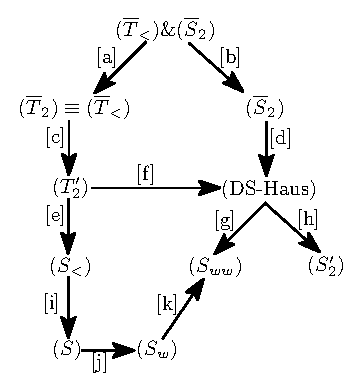
\includegraphics[width=65mm]{../img/Hausdorff_diagram.eps}
  \caption{Hausdorff type axioms}
  \label{fig:haus-diagram}
\end{figure}

\begin{prop}
  The implications $[a]-[k]$ in figure~\ref{fig:haus-diagram} hold.
\end{prop}
\begin{proof}

  [a], [b], [c], [d]:
  trivial.

  [e], [f]:
  from \ref{prop:T2'=DS-Haus+S<}.

  [g]:
  For the sake of contradiction, let $p$ be semiprime yet not prime.
  Thus, there are $x_1, x_2 \ne p$ with $x_1 \wedge x_2 = p$, which means
  $x_1\not\le x_2$ and $x_1\not\ge x_2$.
  Therefore, $x_1 \vee x_2 \not\in \{ x_1, x_2 \}$, and using weakly Hausdorff
  property there exist $u\not\le x_1, v\not\le x_2$ with $u \wedge v = 0$.
  Hence, $u, v\not\le x_1 \wedge x_2 = p$, contradicting the semiprimeness
  of~$p$.

  [h]:
  trivial.

  [i]:
  For the sake of contradiction, consider a~semiprime~$p$ that is not a~coatom,
  that is, $p < a < 1$ for some $a$.
  By~$(S_<)$ we obtain $u\not\le a, v\not\le p$ such that $u \wedge v = 0$.
  Hence, using semiprimeness, $u \le p$ and thus $u < a$, a~contradiction.

  [j], [k]:
  from \ref{prop:S->Sw->Sww}.
\end{proof}

\section{Adding the subfitness}

Subfitness cause $(\overline{S}_2), (S_2'), (\overline{T}_2), (T_2')$ and
(DS-Haus) to coincide as it is seen from

\begin{thm} \label{thm:what-does-sfit-do}
  $(S_2')\&\text{(Sfit)}$ implies $(\overline{S}_2)\&(T_<)$.
\end{thm}

\begin{lem} \label{lem:S2'+Sfit->DSHaus}
  $(S_2')\&\text{(Sfit)}$ implies (DS-Haus).
\end{lem}
\begin{proof}
  Let $a \vee b\not\in \{ a, b \}$.
  Firstly, $a\not\ge b$ means $a \ne 1$.

  Secondly, since $a\not\le b$, by subfitness we have some $c$ with $a \vee c =
  1 \ne b \vee c$.
  Thus, $a\not\le b \vee c$ (otherwise $b \vee c \ge a \vee c = 1$) and again
  $b \vee c \ne 1$.

  As also $a \vee (b \vee c) = 1$, by $(S_2')$ we get $u\not\le a$ and
  $v\not\le b \vee c$ (leading to $v\not\le b$) such that $u \wedge v = 0$.
\end{proof}

\begin{lem} \label{lem:DSHaus+Sfit->overline S}
  (DS-Haus)$\&$(Sfit) implies $(\overline{S}_2)$.
\end{lem}
\begin{proof}
  Let $a\not\le b$ and $a\not\ge b$.
  By (Sfit) we have $c_1, c_2$ such that $a \vee c_1 = 1 \ne b \vee c_1$ and $a
  \vee c_2 \ne 1 = b \vee c_2$.
  Furthermore, if $b \vee c_1 \le a \vee c_2$ then $b \le a \vee c_2$, and
  consequently, $1 = b \vee c_2 \le a \vee c_2$;
  thus $b \vee c_1 \not\le a \vee c_2$ and symmetrically $b \vee c_1 \not\ge a
  \vee c_2$.

  By (DS-Haus) we get $u'\not\le a \vee c_2$ and $v'\not\le b \vee c_1$ such
  that $u' \wedge v' = 0$.

  Finally, set $u := u' \wedge b$ and $v := v' \wedge a$.
  We see that $u\not\le a$ since otherwise $u' = u' \wedge 1 = u' \wedge (b
  \vee c_2) = (u' \wedge b) \vee (u' \wedge c_2) \le a \vee c_2$.
  Likewise, $v\not\le b$.
\end{proof}

\begin{lem} \label{lem:overline S2+Sfit->T<}
  $(\overline{S}_2)\&\text{(Sfit)}$ implies $(T_<)$.
\end{lem}
\begin{proof}
  Let $1 \ne a > b$.
  Once more, by (Sfit) we have $c$ with $a \vee c = 1 \ne b \vee c$.
  Because $a \vee (b \vee c) = 1 \not\in \{ a, b \vee c \}$, we can apply
  $(\overline{S}_2)$ to $a$ and $b \vee c$, thus obtaining $u, v$ such that
  $u\not\le a, v\not\le b \vee c$ (implying $v\not\le b$), $v \le a$ and $u
  \wedge v = 0$.
\end{proof}

\begin{proof}[Proof of~{\bf \ref{thm:what-does-sfit-do}}]
  Use lemmata \ref{lem:S2'+Sfit->DSHaus}, \ref{lem:DSHaus+Sfit->overline S} and
  \ref{lem:overline S2+Sfit->T<}.
\end{proof}
